% !TEX program = lualatex
\RequirePackage{luatex85}
\PassOptionsToPackage{unicode}{hyperref}
\PassOptionsToPackage{naturalnames}{hyperref}
\documentclass{article}
\usepackage{geometry}
%\usepackage{fullpage}
\usepackage{parskip}
\usepackage{physics}
\usepackage{amsmath}
\usepackage{amssymb}
\usepackage{xcolor}
\usepackage[colorlinks,linkcolor=blue,citecolor=green]{hyperref}
\usepackage{array}
\usepackage{longtable}
\usepackage{multirow}
\usepackage{comment}
\usepackage{graphicx}
\usepackage{cite}
\usepackage{amsfonts}
\usepackage{bm}
\usepackage{slashed}
\usepackage{dsfont}
\usepackage{mathtools}
\usepackage[compat=1.1.0]{tikz-feynman}
\usepackage{simplewick}
\usepackage{mathrsfs}
\usepackage{xparse}
\usepackage{enumerate}
\usepackage{extarrows}

\allowdisplaybreaks

\newcommand{\calA}{\mathcal{A}}
\newcommand{\mm}[1]{\frac{\dd^4#1}{(2\pi)^4}}
\newcommand{\mme}[1]{\frac{\dd^3\vb{#1}}{(2\pi)^3}}

\title{Note on Braaten's Paper}
\author{Yingsheng Huang}
\begin{document}
    \maketitle
    
    \section{Intro}
    Hamiltonian\cite{Braaten2008}: 
    \begin{align}
        \mathcal{H}=\sum_\sigma\frac{1}{2m}\nabla\psi_\sigma^{\dagger}\cdot\nabla\psi_\sigma^{(\Lambda)}+\frac{g(\Lambda)}{m}\psi^\dagger_1\psi^\dagger_2\psi_3\psi_4^{(\Lambda)}+\mathcal{V}
    \end{align}
    where the renormalized coupling 
    \begin{align}
        g(\Lambda)=\frac{4\pi a}{1-2a\Lambda/\pi}
        \label{gL}
    \end{align}

    \section{Amplitude}
    Consider: 
    \begin{align}
        i\calA=\mel{34}{\psi^\dagger\psi}{12}=
        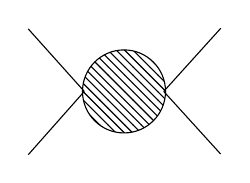
\begin{tikzpicture}[baseline=(o1.base)]
            \begin{feynman}
                \diagram[small,horizontal=o1 to o3]{
                    p1 -- o1 --[draw=none] o3 -- p3;
                    p2 -- o1 --[draw=none] o3 -- p4;
                };
                \node[blob, minimum size=30pt] at ($(o1)!0.5!(o3)$) (o2);
            \end{feynman}
        \end{tikzpicture}
    \end{align}
    Define $P=p_1+p_2=(E,\vb{0})$, and $E=p^2/m$. 
    The integral equation is 
    \begin{align}
        i\calA=-\frac{ig(\Lambda)}{m}\pqty{1+i\calA\int\mm{k}\frac{i}{k^0-\frac{\vb{k}^2}{2m}+i\epsilon}\frac{i}{k^0-p^0-\frac{\abs{\vb{k-p}}^2}{2m}+i\epsilon}}
    \end{align}
    The integral gives (redefine $\epsilon\rightarrow2m\epsilon$)
    \begin{align}
        \mathcal{I}=\frac{i m }{2 \pi ^2}\left(-\Lambda +\sqrt{ -mE-i \epsilon } \tan ^{-1}\left(\frac{\Lambda }{\sqrt{ -mE-i \epsilon }}\right)\right)=-\frac{i \Lambda  m}{2 \pi ^2}+\frac{m p}{4 \pi }
    \end{align}
    and 
    \begin{align}
        i\calA&=\frac{-1}{\mathcal{I}+\frac{m}{ig(\Lambda)}}=-\bqty{\frac{i m \sqrt{-mE -i \epsilon } \tan ^{-1}\left(\frac{\Lambda }{\sqrt{-mE -i \epsilon }}\right)}{2 \pi ^2}-\frac{i m}{4 \pi  a}}^{-1}\\
        &\xlongequal{\Lambda\rightarrow\infty}\frac{4 i \pi/m  }{-1/a+ \sqrt{-mE -i \epsilon }}
    \end{align}

    Note that by definition, scattering length is the leading order momentum expansion of $1/\calA$, which gives 
    \begin{align}
        \frac{1}{a}&=\frac{4i\pi}{m}\pqty{\mathcal{I}+\frac{m}{ig(\Lambda)}}^{(0)}\\
        &=\frac{4 \pi }{g(\Lambda)}+\frac{2 \Lambda }{\pi }\\
        &\hspace{-0.4in}\Rightarrow g(\Lambda)=\frac{4 \pi  a}{1 -2 a \Lambda/\pi }
    \end{align}
    and this is actually how we get the form of \eqref{gL}. 

    \section{OPE}
    \subsection{l.h.s.}
    Take what we got in the last section as a new non-perturbative vertex, we only need to deal with tree diagram this way. First we have Figure~2(a) in Braaten's paper: 
    \begin{align}
        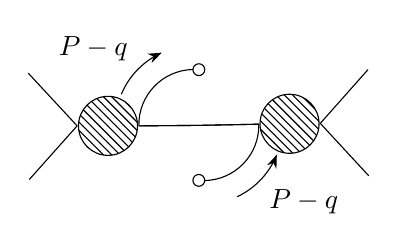
\begin{tikzpicture}[baseline=(o1.base)]
            \begin{feynman}
                \diagram[small,horizontal=o1 to o3]{
                    p1 -- o1 --[draw=none] o3 -- o35 -- o4 --[draw=none] o6 -- p3;
                    p2 -- o1 --[draw=none] o3 -- o35 -- o4 --[draw=none] o6 -- p4;
                };
                \node[empty dot] at ($(o3)!0.5!(o4)+(0,20pt)$) (ps1);
                \node[empty dot] at ($(o3)!0.5!(o4)+(0,-20pt)$) (ps2);
                \diagram*{
                    (o3) --[quarter left,momentum={[arrow shorten=0.25]\(P-q\)}] (ps1);
                    (ps2) --[quarter right,momentum'={[arrow shorten=0.25]\(P-q\)}] (o4);
                };
                \node[blob] at ($(o1)!0.5!(o3)$) (o2);
                \node[blob] at ($(o4)!0.5!(o6)$) (o5);
            \end{feynman}
        \end{tikzpicture}&=\mel{34}{\psi^\dagger\left(-\frac{\vb{r}}{2}\right)\psi\left(\frac{\vb{r}}{2}\right)}{12}\\
        &=(i\calA)^2\int\frac{\dd^4q}{(2\pi)^4}\frac{i}{q^0-\frac{\vb{q}^2}{2m}+i\epsilon}\frac{i}{\bqty{E-q^0-\frac{\vb{q}^2}{2m}+i\epsilon}^2}e^{i\vb{q}\cdot\vb{r}}\\
        &=\calA^2\int\frac{\dd^3\vb{q}}{(2\pi)^3}\frac{m^2e^{i\vb{q}\cdot\vb{r}}}{\pqty{\vb{q}^2-p^2-i\epsilon}^2}\\
        &=\frac{i m^2\calA^2 e^{i p r}}{8 \pi  p}
    \end{align}
    \subsection{r.h.s.}
    For simplicity, we drop the external lines and focus on the internal subgraph. Consider Figure~2(b):
    \begin{align}
        &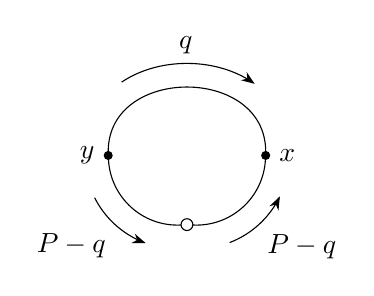
\begin{tikzpicture}[baseline=(o3.base)]
            \begin{feynman}
                \diagram[small,horizontal=o3 to o4,layered layout]{
                    o3[dot,label=180:\(y\)] --[draw=none] o35 --[draw=none] o4[dot,label=0:\(x\)];
                };
                \vertex at ($(o3)!0.5!(o4)+(0,25pt)$) (ps1);
                \node[empty dot] at ($(o3)!0.5!(o4)+(0,-25pt)$) (ps2);
                \diagram*{
                    (o3) --[half left,looseness=1.4,momentum={[arrow shorten=0.25]\(q\)}] (o4);
                    (o3) --[quarter right,momentum'={[arrow shorten=0.25]\(P-q\)}] (ps2);
                    (ps2) --[quarter right,momentum'={[arrow shorten=0.25]\(P-q\)}] (o4);
                };
            \end{feynman}
        \end{tikzpicture}=\mel{34}{\psi^\dagger\psi\left(0\right)}{12}_{amp}\\
        &=\int\dd^4x\int\dd^4y\int\mm{l_1}\mm{l_2}\mm{q}e^{iP\cdot y}e^{-iP\cdot x}e^{-il_1\cdot y}e^{il_2\cdot x}e^{iq\cdot (x-y)}\tilde D(l_1)\tilde D(l_2)\tilde D(q)\\
        &=\int\mm{q}\tilde D(P-q)\tilde D(P-q)\tilde D(q)\\
        &=-\int\mme{q}\frac{m^2}{\pqty{\vb{q}^2-p^2-i\epsilon}^2}\\
        &=-\frac{im^2}{8\pi p}
    \end{align}
    where $\tilde D$ marks momentum space propagator and two external vertexes give an $(i\calA)^2$ factor. The total contribution is 
    \begin{align}
        \frac{im^2\calA^2}{8\pi p},
    \end{align}
    the first order Fourier expansion of the l.h.s. 
    \subsection{Higher dimensional operators}
    Figure~2(c) gives
    \begin{align}
        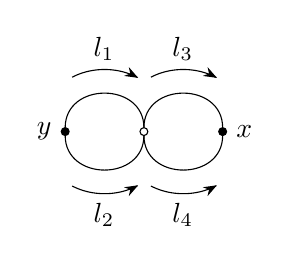
\begin{tikzpicture}[baseline=(o3.base)]
            \begin{feynman}
                \diagram[small,horizontal=o3 to o4,layered layout]{
                    o3[dot,label=180:\(y\)] --[half left,momentum={[arrow shorten=0.3]\(l_1\)}] o35[empty dot] --[half left,momentum={[arrow shorten=0.3]\(l_3\)}] o4[dot,label=0:\(x\)];
                    o3 --[half right,momentum'={[arrow shorten=0.3]\(l_2\)}] o35 --[half right,momentum'={[arrow shorten=0.3]\(l_4\)}] o4;
                };
            \end{feynman}
        \end{tikzpicture}&=\mel{34}{\psi^\dagger\psi^\dagger\psi\psi\left(0\right)}{12}_{amp}\\
        &=\int\dd^4x\int\dd^4y\int\mm{l_1}\mm{l_2}\mm{l_3}\mm{l_4}e^{iP\cdot y}e^{-iP\cdot x}e^{-i(l_1+l_2)\cdot y}e^{i(l_3+l_4)\cdot x}\notag\\
        &\tilde D(l_1)\tilde D(l_2)\tilde D(l_3)\tilde D(l_4)
    \end{align}
    which becomes
    \begin{align}
        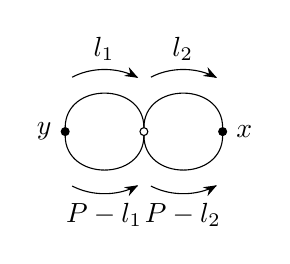
\begin{tikzpicture}[baseline=(o3.base)]
            \begin{feynman}
                \diagram[small,horizontal=o3 to o4,layered layout]{
                    o3[dot,label=180:\(y\)] --[half left,momentum={[arrow shorten=0.3]\(l_1\)}] o35[empty dot] --[half left,momentum={[arrow shorten=0.3]\(l_2\)}] o4[dot,label=0:\(x\)];
                    o3 --[half right,momentum'={[arrow shorten=0.3]\(P-l_1\)}] o35 --[half right,momentum'={[arrow shorten=0.3]\(P-l_2\)}] o4;
                };
            \end{feynman}
        \end{tikzpicture}&=\int\mm{l_1}\mm{l_2}\tilde D(l_1)\tilde D(P-l_1)\tilde D(l_2)\tilde D(P-l_2)\\
        &=-\int\mme{l_1}\mme{l_2}\frac{m^2}{\left(\vb{l_1}^2-p^2-i \epsilon \right) \left(\vb{l_2}^2-p^2-i \epsilon \right)}\\
        &=-\mathcal{I}^2
    \end{align}
    There're four diagrams in total: 
    \begin{align}
        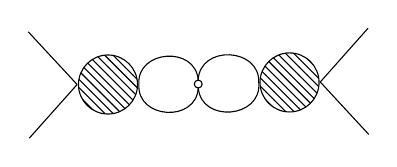
\begin{tikzpicture}[baseline=(o1.base)]
            \begin{feynman}
                \diagram[small,horizontal=o1 to o3]{
                    p1 -- o1 --[draw=none] o3 --[draw=none] o35[empty dot] --[draw=none] o4 --[draw=none] o6 -- p3;
                    p2 -- o1 --[draw=none] o3 --[draw=none] o35 --[draw=none] o4 --[draw=none] o6 -- p4;
                };
                \diagram*{
                    (o3) --[half left] (o35) --[half left] (o4);
                    (o3) --[half right] (o35) --[half right] (o4);
                };
                \node[blob] at ($(o1)!0.5!(o3)$) (o2);
                \node[blob] at ($(o4)!0.5!(o6)$) (o5);
            \end{feynman}
        \end{tikzpicture}&=\calA^2\mathcal{I}^2\\
        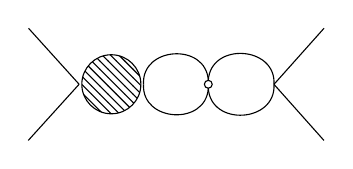
\begin{tikzpicture}[baseline=(o1.base)]
            \begin{feynman}
                \diagram[small,horizontal=o1 to o3]{
                    p1 -- o1 --[draw=none] o3 --[draw=none] o35[empty dot] --[draw=none] o4 -- p3;
                    p2 -- o1 --[draw=none] o3 --[draw=none] o35 --[draw=none] o4 -- p4;
                };
                \diagram*{
                    (o3) --[half left] (o35) --[half left] (o4);
                    (o3) --[half right] (o35) --[half right] (o4);
                };
                \node[blob] at ($(o1)!0.5!(o3)$) (o2);
            \end{feynman}
        \end{tikzpicture}&=\calA\mathcal{I}\\
        \begin{tikzpicture}[baseline=(o1.base)]
            \begin{feynman}
                \diagram[small,horizontal=o3 to o4]{
                    p1 -- o3 --[draw=none] o35[empty dot] --[draw=none] o4 --[draw=none] o6 -- p3;
                    p2 -- o3 --[draw=none] o35 --[draw=none] o4 --[draw=none] o6 -- p4;
                };
                \diagram*{
                    (o3) --[half left] (o35) --[half left] (o4);
                    (o3) --[half right] (o35) --[half right] (o4);
                };
                \node[blob] at ($(o4)!0.5!(o6)$) (o5);
            \end{feynman}
        \end{tikzpicture}&=\calA\mathcal{I}\\
        \begin{tikzpicture}[baseline=(o1.base)]
            \begin{feynman}
                \diagram[small,horizontal=o3 to o4]{
                    p1 -- o3 --[draw=none] o35[empty dot] --[draw=none] o4 -- p3;
                    p2 -- o3 --[draw=none] o35 --[draw=none] o4 -- p4;
                };
                \diagram*{
                    (o3) --[half left] (o35) --[half left] (o4);
                    (o3) --[half right] (o35) --[half right] (o4);
                };
            \end{feynman}
        \end{tikzpicture}&=1
    \end{align}
    We have 
    \begin{align}
        \expval{\psi^\dagger_1\psi^\dagger_2\psi_1\psi_2^{(\Lambda)}(0)}_{\pm\vb{p}}=(\calA\mathcal{I}+1)^2
    \end{align}
    in total. Plug in 
    \begin{align}
        \mathcal{I}=-\frac{m}{ig(\Lambda)}-\frac{1}{\calA}
    \end{align}
    we have
    \begin{align}
        \expval{\psi^\dagger_1\psi^\dagger_2\psi_1\psi_2^{(\Lambda)}(0)}_{\pm\vb{p}}=m^2g^{-2}(\Lambda)\calA^2
        \label{2c}
    \end{align}
    The Wilson coefficient must be 
    \begin{align}
        -\frac{r}{8\pi}g^2(\Lambda)
    \end{align}

    \section{Contact}
    \subsection{Definition}
    \begin{align}
        C=\int\dd^3R\expval{g^2\psi^\dagger_1\psi^\dagger_2\psi_1\psi_2(R)}
    \end{align}
    \subsection{Energy Relation}

    \subsection{OPE for number density operators}
    We have a pair of number density operators
    \begin{align}
        \psi_1^\dagger\psi_1(\vb{R}-\frac{1}{2}\vb{r})\;\&\; \psi_2^\dagger\psi_2(\vb{R}+\frac{1}{2}\vb{r})
    \end{align}
    and the diagram is 
    \begin{align}
        &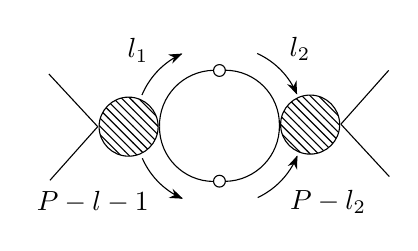
\begin{tikzpicture}[baseline=(o1.base)]
            \begin{feynman}
                \diagram[small,horizontal=o1 to o3]{
                    p1 -- o1 --[draw=none] o3 --[draw=none] o35 --[draw=none] o4 --[draw=none] o6 -- p3;
                    p2 -- o1 --[draw=none] o3 --[draw=none] o35 --[draw=none] o4 --[draw=none] o6 -- p4;
                };
                \node[empty dot] at ($(o3)!0.5!(o4)+(0,20pt)$) (ps1);
                \node[empty dot] at ($(o3)!0.5!(o4)+(0,-20pt)$) (ps2);
                \diagram*{
                    (o3) --[quarter left,momentum={[arrow shorten=0.25]\(l_1\)}] (ps1);
                    (ps1) --[quarter left,momentum={[arrow shorten=0.25]\(l_2\)}] (o4);
                    (o3) --[quarter right,momentum'={[arrow shorten=0.25]\(P-l-1\)}] (ps2);
                    (ps2) --[quarter right,momentum'={[arrow shorten=0.25]\(P-l_2\)}] (o4);
                };
                \node[blob] at ($(o1)!0.5!(o3)$) (o2);
                \node[blob] at ($(o4)!0.5!(o6)$) (o5);
            \end{feynman}
        \end{tikzpicture}\\
        &=(i\calA)^2\int\mm{l_1}\mm{l_2}\frac{i}{l_1^0-\frac{\vb{l_1}^2}{2m}+i\epsilon}\frac{i}{{E-l_1^0-\frac{\vb{l_1}^2}{2m}+i\epsilon}}\frac{i}{l_2^0-\frac{\vb{l_2}^2}{2m}+i\epsilon}\frac{i}{{E-l_2^0-\frac{\vb{l_2}^2}{2m}+i\epsilon}}e^{i\vb{q}\cdot\vb{r}}\\
        &=\frac{\calA^2m^2 }{16 \pi ^2 r^2}e^{2 i p r}
    \end{align}
    Compare with the result of Figure~2(c) \eqref{2c} we have the Wilson coefficient
    \begin{align}
        \frac{g^2(\Lambda)}{16 \pi ^2 r^2}
    \end{align}

    \bibliography{../../QM-OPE/QM-OPE.bib}
    \bibliographystyle{apsrev4-1}
\end{document}